\section[\appendixname~\thesection]{Representative Trajectory Case: \texttt{BLAN} to \texttt{WOHL}}
\label{sec:blan_wohl_trajectory}

This appendix shows one example request from start to end, so that it is clear what the planner pipeline of Section~\ref{sec:methodology} produces before the runtime and conflict results of Section~\ref{sec:results}. It is not needed to follow those results. The request goes from vertiport \texttt{BLAN} to vertiport \texttt{WOHL}; here and below, four-letter codes in typewriter font are the identifiers of the Hamburg vertiports in Figure~\ref{fig:hamburg_corridor_network}. The request uses the fixed cruise layer of \SI{200}{m} MSL and does not call the Deconfliction Service. We chose this case because it uses several corridor segments and the departure, cruise and arrival phases are clearly visible. For this pair, A* selects the corridor sequence
\[
\texttt{BLAN} \rightarrow \texttt{VOLK} \rightarrow \texttt{SCHN} \rightarrow
\texttt{FUHB} \rightarrow \texttt{WOHL}.
\]

Figure~\ref{fig:blan_wohl_paths_overview} shows this route in the Hamburg corridor graph. The thin blue edges are the available corridor connections, the red markers are graph nodes, and the thick blue line is the selected A* path from \texttt{BLAN} over \texttt{VOLK}, \texttt{SCHN} and \texttt{FUHB} to \texttt{WOHL}.

\begin{figure}[!htbp]
  \centering
  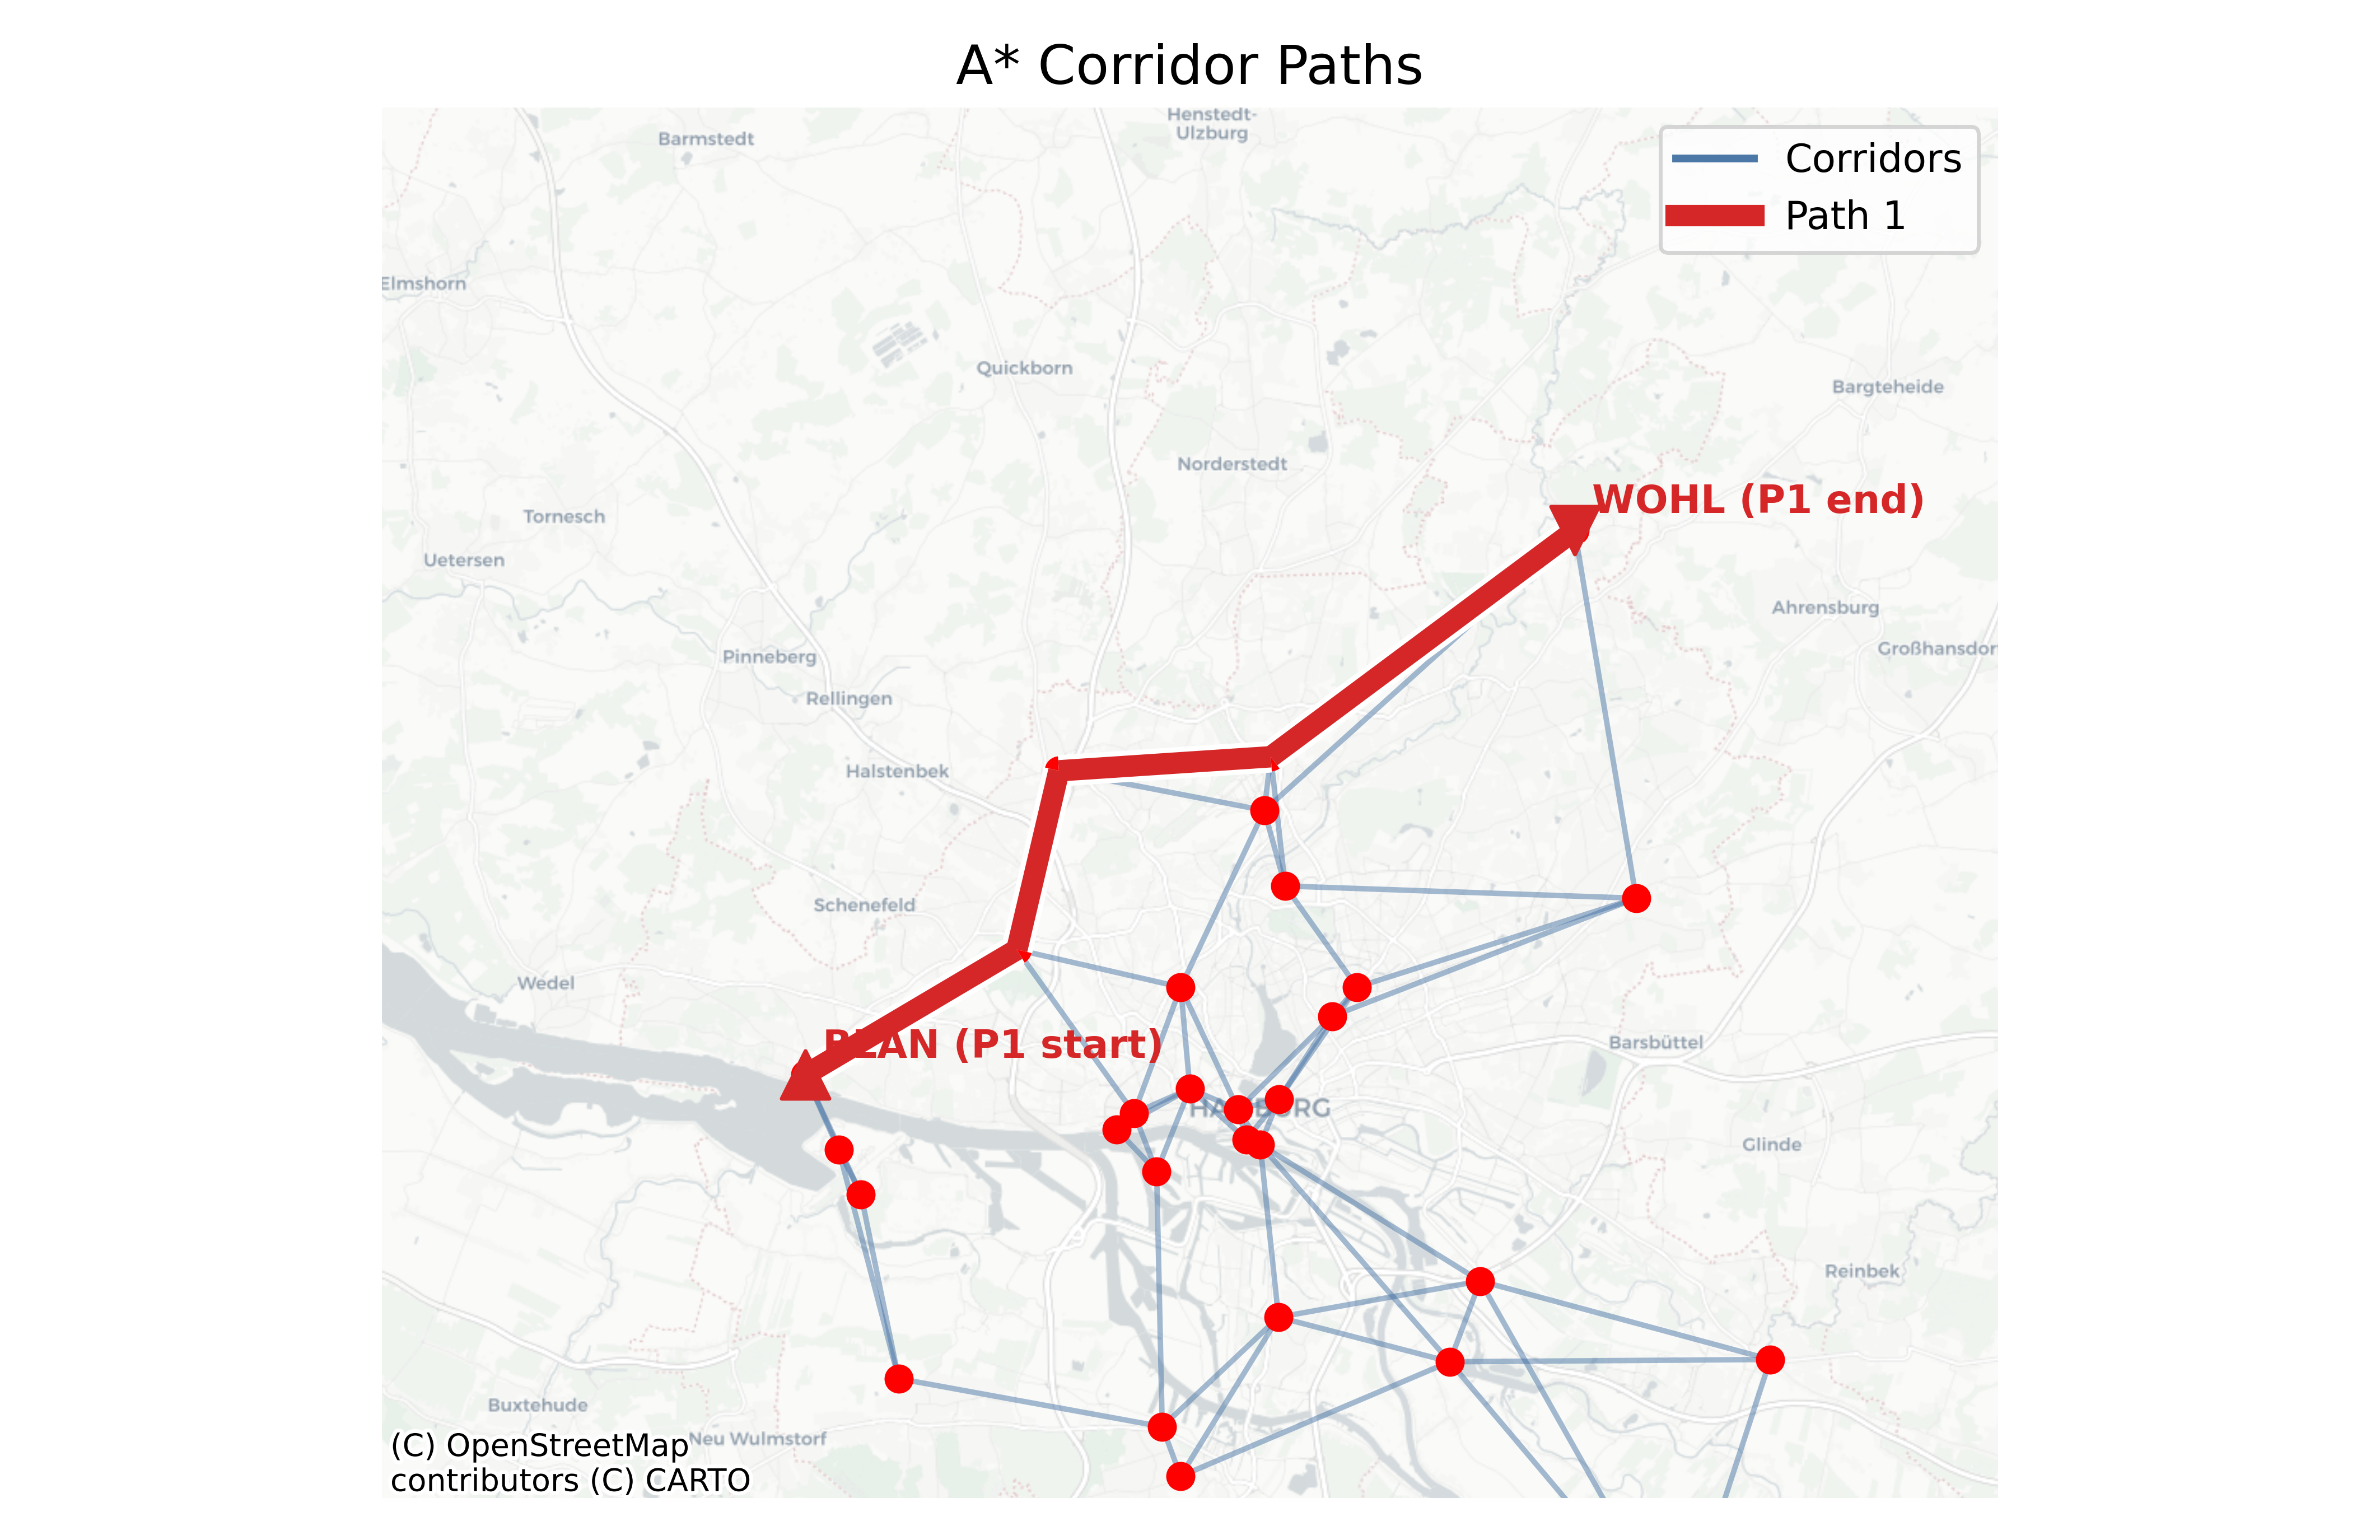
\includegraphics[width=0.95\linewidth]{figures/blan_wohl_paths_overview.png}
  \caption{A* corridor path overview for the \texttt{BLAN} to \texttt{WOHL} request. The highlighted path connects the departure vertiport \texttt{BLAN} with the landing vertiport \texttt{WOHL} through the selected corridor sequence via the intermediate vertiports \texttt{VOLK}, \texttt{SCHN}, and \texttt{FUHB}.}
  \label{fig:blan_wohl_paths_overview}
\end{figure}

The waypoint synthesizer turns this five-node route into 11 CFMS input waypoints for departure, transition, cruise, top of descent and landing. The three cruise nodes \texttt{VOLK}, \texttt{SCHN} and \texttt{FUHB} are kept as centerline references. The resulting trajectory has 1713 samples at about \SI{1}{s} spacing, a distance of \SI{27.99}{km} along the track, and a duration of \SI{1596.74}{s}, or \SI{26.61}{min}.

The speed stored with each trajectory sample is the horizontal speed of the aircraft: it follows the change of the along-track distance and is exactly zero during the purely vertical climb and descent, even though the aircraft is moving vertically there. We therefore call it \emph{horizontal speed} in this paper. Since no wind is modeled, horizontal airspeed and ground speed are the same here. The simple mean of the speed samples over this trajectory is \SI{17.15}{m/s}, while distance divided by duration gives \SI{17.53}{m/s}. The difference comes from the sampling: the samples are not evenly spaced in time---the terminal phases have more samples than cruise---so the simple mean gives too much weight to the slow terminal segments. If each sample is weighted by its time step, the mean is exactly \SI{17.53}{m/s}. In cruise the speed is about \SI{25}{m/s}.

Figure~\ref{fig:blan_wohl_map} shows the lateral trajectory in three phase panels. The panels are split at corridor nodes: the first panel, \emph{departure and outbound climb}, goes from the origin pad to the first corridor node and so includes the whole outbound leg to \texttt{VOLK}, not only the take-off procedure; in the same way, the \emph{inbound descent and arrival} panel goes from the last corridor node \texttt{FUHB} to the destination pad. The first climb is flown almost vertically over the pad, so the track leaves \texttt{BLAN} straight in the outbound corridor direction, without a turn at low height around waypoint~1. The cruise panel shows the route over \texttt{VOLK}, \texttt{SCHN} and \texttt{FUHB}, and the arrival panel ends with a vertical descent over the destination pad. So the generated trajectory follows the A* corridor sequence and adds the terminal geometry at both ends. The altitude and speed profiles are shown in Figures~\ref{fig:blan_wohl_altitude} and~\ref{fig:blan_wohl_speed}.

\begin{figure}[!htbp]
  \centering
  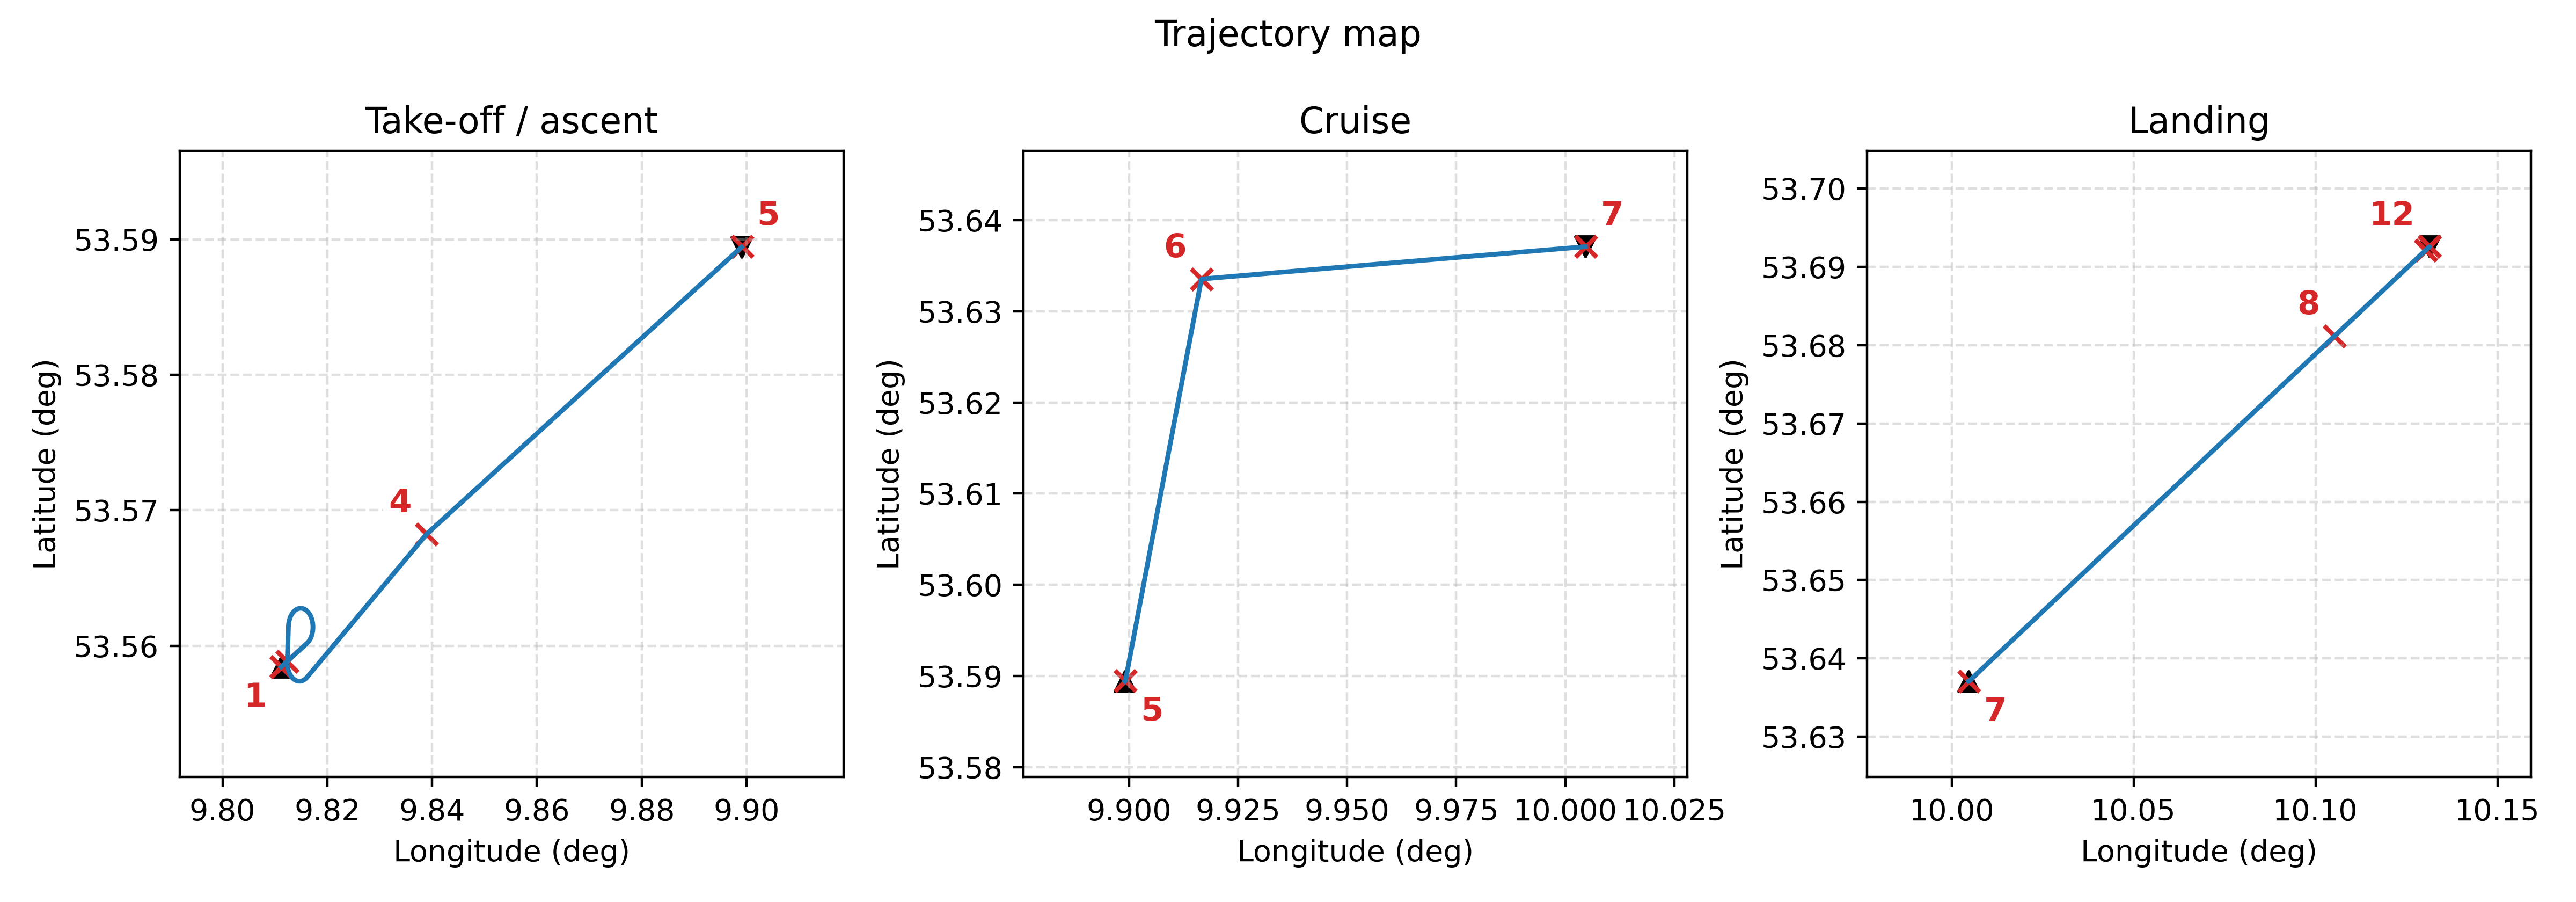
\includegraphics[width=0.92\linewidth]{figures/blan_wohl_trajectory_map.png}
  \caption{Phase-separated lateral trajectory for the \texttt{BLAN} to \texttt{WOHL} request. Red numbered markers indicate synthesized CFMS waypoints in sequence order; the blue line is the generated trajectory; black triangles mark each panel's start and end points. The panels separate the departure and outbound climb (pad to first corridor node), the corridor cruise portion, and the inbound descent and arrival (last corridor node to pad). Boundary waypoints are repeated across adjacent panels to show phase continuity.}
  \label{fig:blan_wohl_map}
\end{figure}

Figure~\ref{fig:blan_wohl_altitude} shows the altitude profile. Each of the three panels has its own time axis starting at zero, so each phase can be seen at a useful scale. At departure, the aircraft first climbs vertically through the lower terminal height and then climbs steeply along the outbound leg up to the outer-limitation-surface reference at \SI{152}{m}. It holds this height until the first corridor node and then climbs to the \SI{200}{m} MSL cruise layer, which it keeps along the middle corridor segment. On arrival, it descends from the cruise layer to the \SI{152}{m} approach reference shortly after the last corridor segment, holds this level on the inbound leg until the top of descent, and then descends through the \SI{60}{m} and \SI{15}{m} terminal references before the vertical final descent onto the \texttt{WOHL} pad. This shows how waypoint synthesis combines the fixed cruise altitude with the departure and arrival procedures.

\begin{figure}[!htbp]
  \centering
  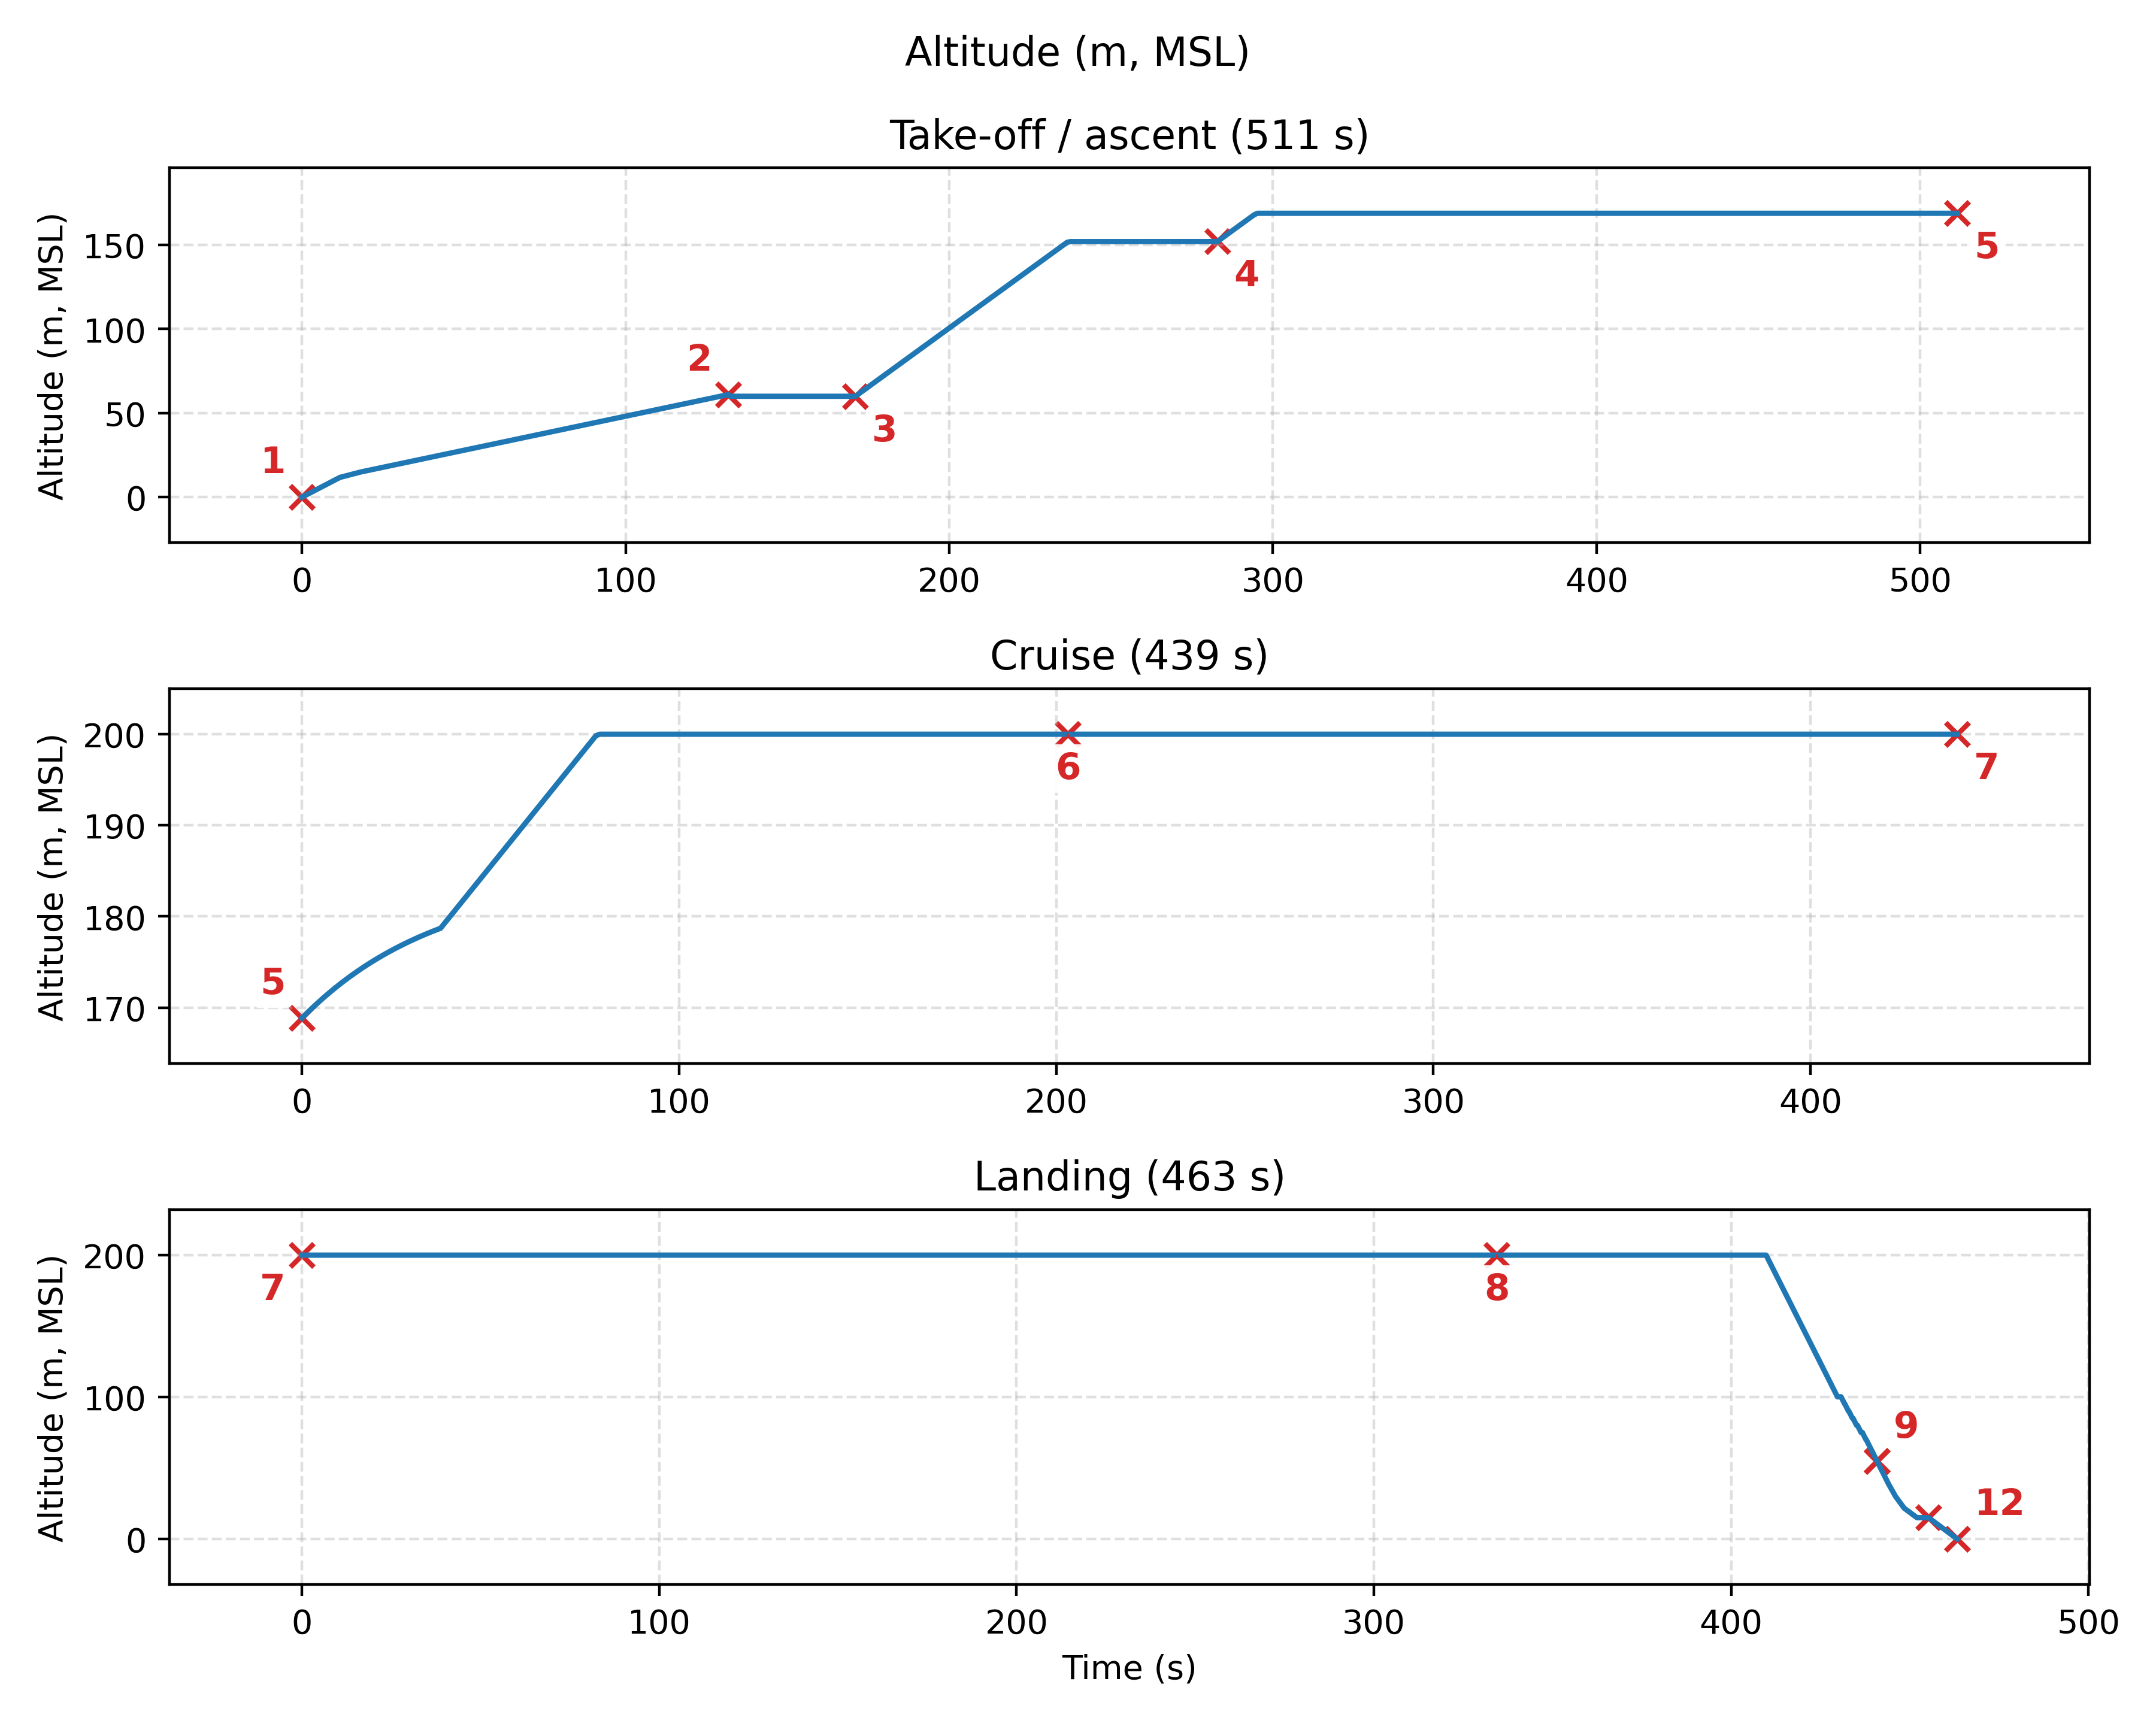
\includegraphics[width=0.74\linewidth]{figures/blan_wohl_trajectory_altitude.png}
  \caption{Altitude profile for the \texttt{BLAN} to \texttt{WOHL} trajectory. The three panels show departure and outbound climb, cruise, and inbound descent and arrival; each panel uses its own phase-relative time axis starting at zero, with the phase duration given in the panel title, so the panels concatenate to the full \SI{1596.74}{s} flight. Red markers are the CFMS input waypoints; the number label is omitted where two markers nearly coincide. The profile reaches the fixed \SI{200}{m} MSL cruise layer before descending into \texttt{WOHL}.}
  \label{fig:blan_wohl_altitude}
\end{figure}

Figure~\ref{fig:blan_wohl_speed} shows the horizontal-speed profile, again with one time axis per phase. The speed starts and ends at zero because the first climb and the last descent are vertical. After lift-off, the aircraft flies the departure funnel at a low constant speed of about \SI{5}{m/s}, speeds up to \SI{20}{m/s} on the outbound leg, and reaches the cruise speed of about \SI{25}{m/s} on the middle corridor segment. On arrival, the speed is reduced step by step through the approach speed limits before the final vertical descent. Whether the aircraft stays inside a corridor volume cannot be concluded from this speed profile; that would need a separate check.

\begin{figure}[!htbp]
  \centering
  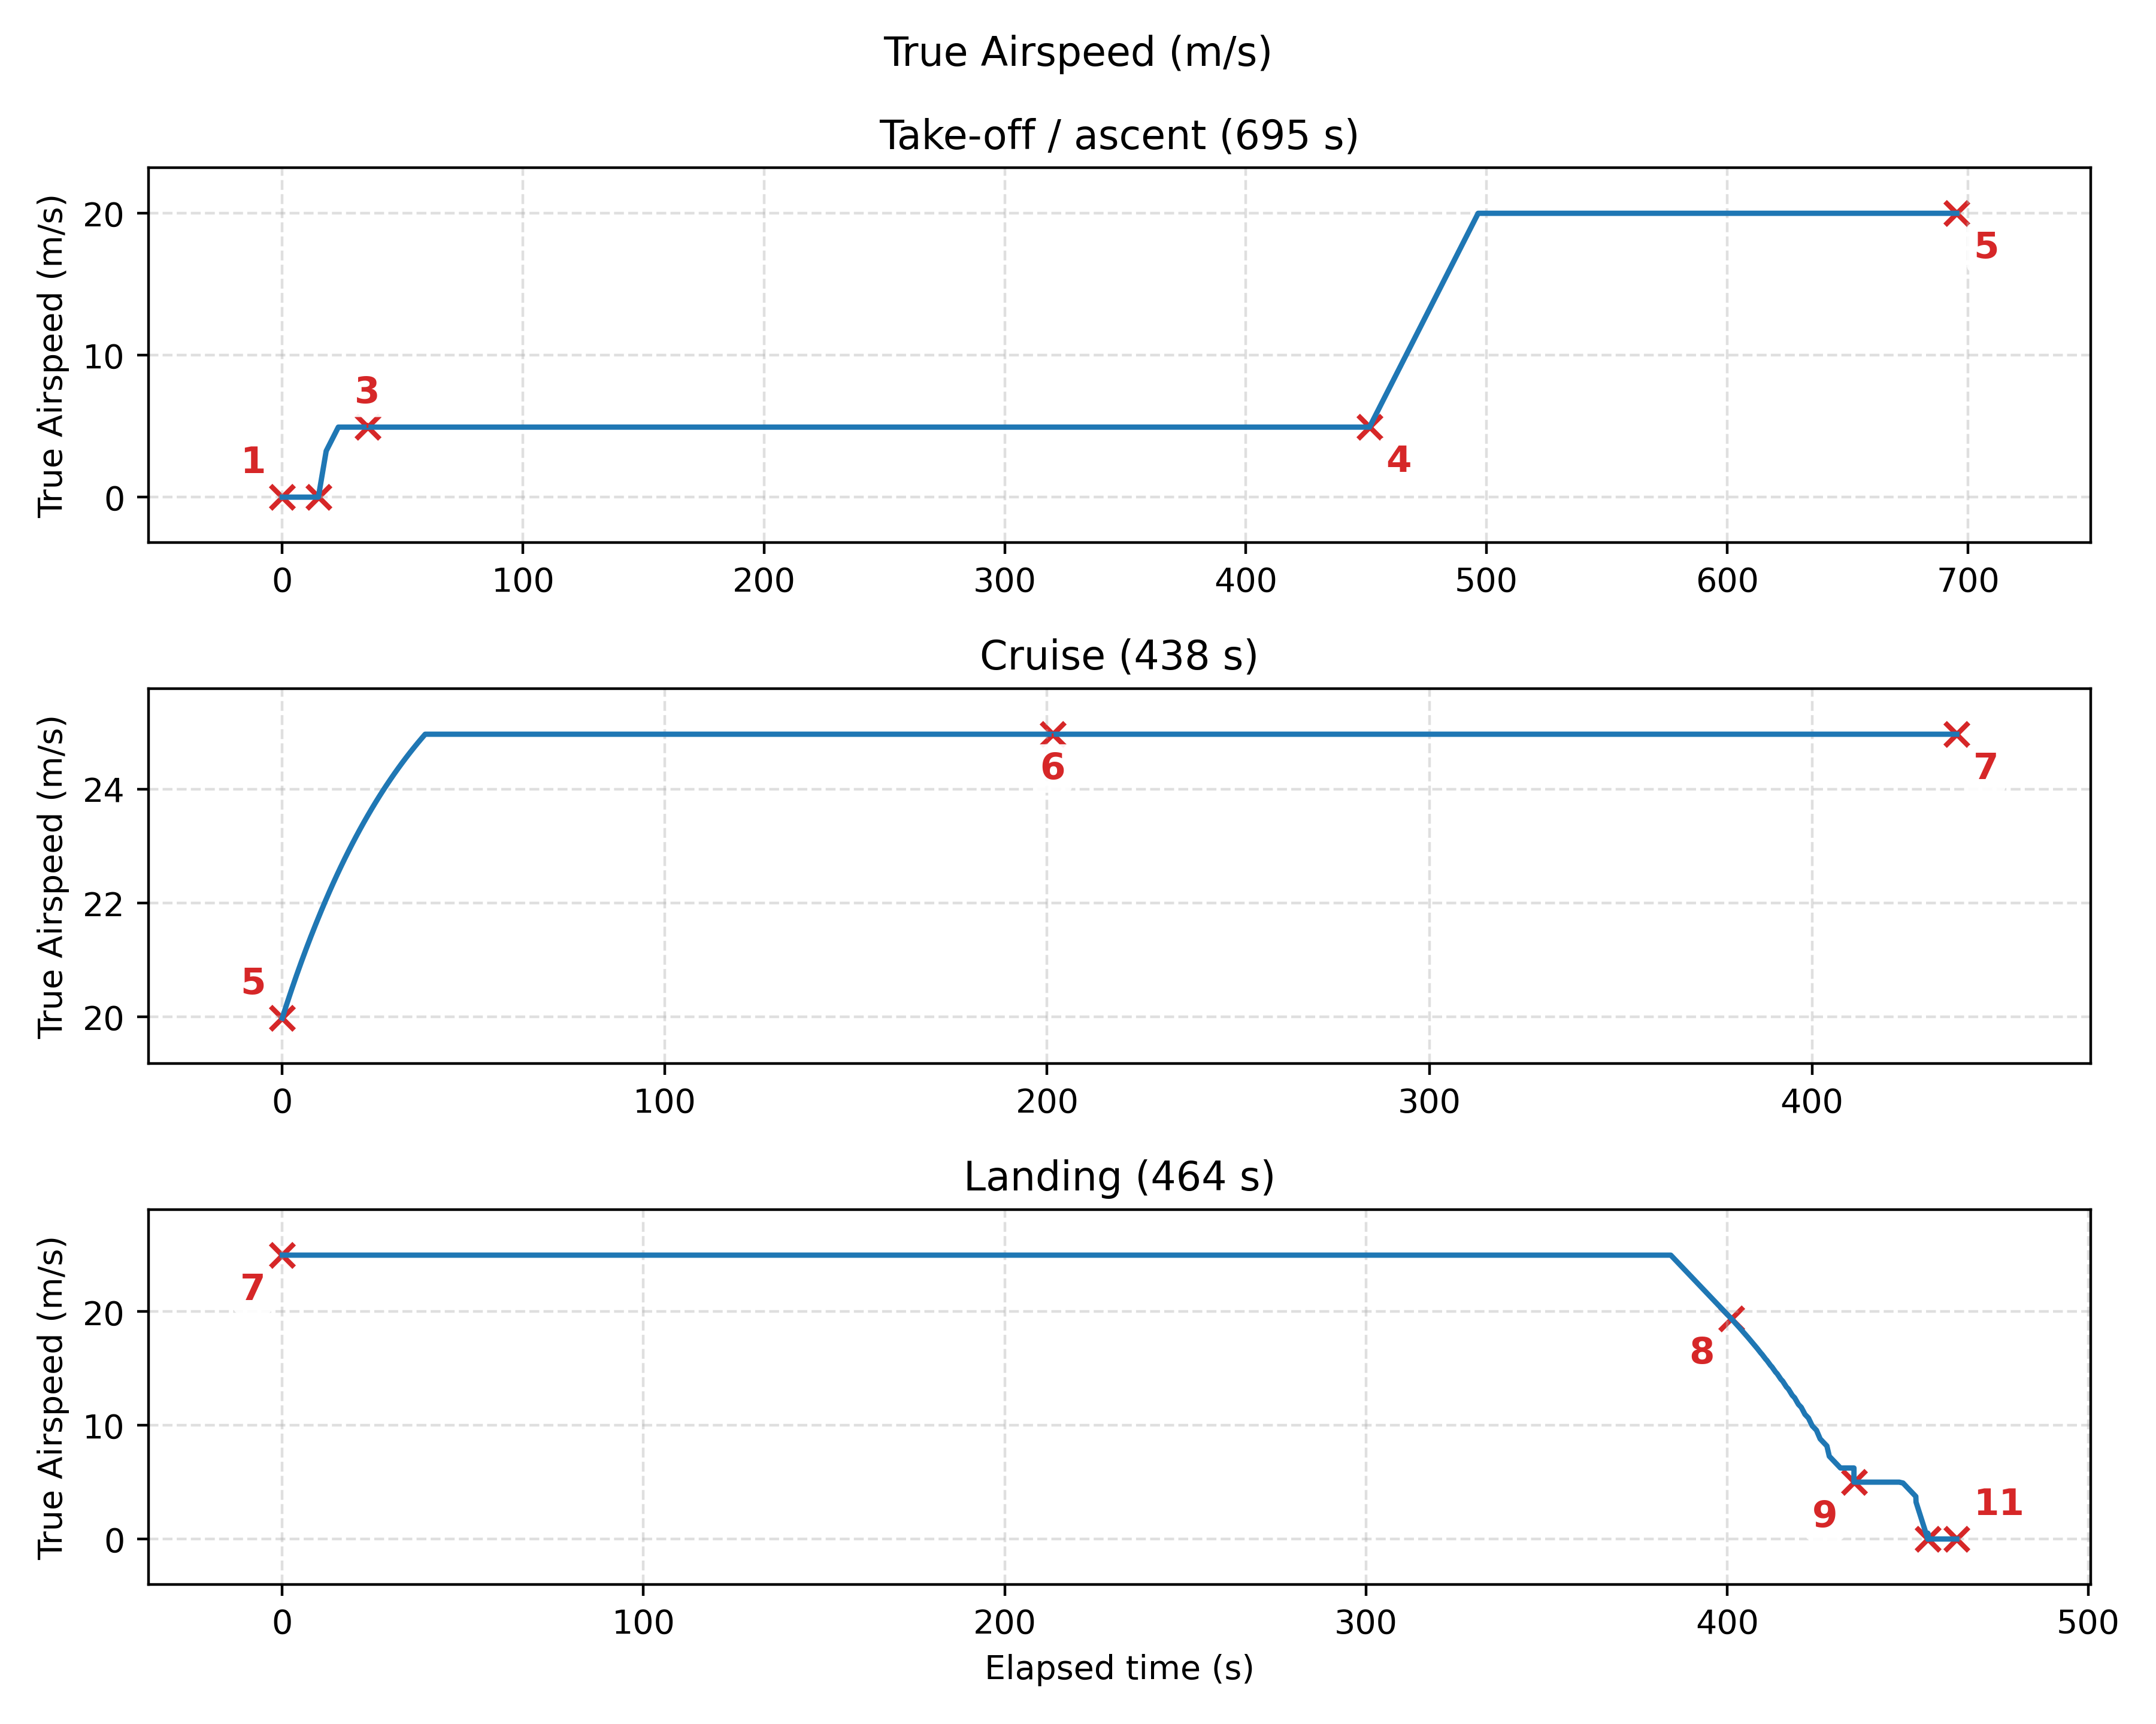
\includegraphics[width=0.74\linewidth]{figures/blan_wohl_trajectory_tas.png}
  \caption{Horizontal-speed profile for the \texttt{BLAN} to \texttt{WOHL} trajectory. The plotted quantity is the speed field reported with each generated trajectory sample, which is the horizontal component only and is zero during purely vertical motion; no wind is modeled, so horizontal airspeed and ground speed coincide here. The phase-separated panels use the same phase-relative time axes as the altitude profile and red markers for the CFMS input waypoints, with the number label omitted where two markers nearly coincide. Visible are the zero-speed vertical lift-off, the \SI{5}{m/s} departure-funnel segment, the acceleration to \SI{20}{m/s} on the outbound leg, the approximately constant \SI{25}{m/s} cruise, and the staged deceleration through the approach speed limits before the vertical final descent.}
  \label{fig:blan_wohl_speed}
\end{figure}
